\documentclass{ximera}


\graphicspath{
  {./}
  {ximeraTutorial/}
  {basicPhilosophy/}
}

\newcommand{\mooculus}{\textsf{\textbf{MOOC}\textnormal{\textsf{ULUS}}}}

\usepackage{tkz-euclide}\usepackage{tikz}
\usepackage{tikz-cd}
\usetikzlibrary{arrows}
\tikzset{>=stealth,commutative diagrams/.cd,
  arrow style=tikz,diagrams={>=stealth}} %% cool arrow head
\tikzset{shorten <>/.style={ shorten >=#1, shorten <=#1 } } %% allows shorter vectors

\usetikzlibrary{backgrounds} %% for boxes around graphs
\usetikzlibrary{shapes,positioning}  %% Clouds and stars
\usetikzlibrary{matrix} %% for matrix
\usepgfplotslibrary{polar} %% for polar plots
\usepgfplotslibrary{fillbetween} %% to shade area between curves in TikZ
\usetkzobj{all}
\usepackage[makeroom]{cancel} %% for strike outs
%\usepackage{mathtools} %% for pretty underbrace % Breaks Ximera
%\usepackage{multicol}
\usepackage{pgffor} %% required for integral for loops



%% http://tex.stackexchange.com/questions/66490/drawing-a-tikz-arc-specifying-the-center
%% Draws beach ball
\tikzset{pics/carc/.style args={#1:#2:#3}{code={\draw[pic actions] (#1:#3) arc(#1:#2:#3);}}}



\usepackage{array}
\setlength{\extrarowheight}{+.1cm}
\newdimen\digitwidth
\settowidth\digitwidth{9}
\def\divrule#1#2{
\noalign{\moveright#1\digitwidth
\vbox{\hrule width#2\digitwidth}}}






\DeclareMathOperator{\arccot}{arccot}
\DeclareMathOperator{\arcsec}{arcsec}
\DeclareMathOperator{\arccsc}{arccsc}

















%%This is to help with formatting on future title pages.
\newenvironment{sectionOutcomes}{}{}


\title{Projectile Motion}

\begin{document}

\begin{abstract}
%Stuff can go here later if we want!
\end{abstract}
\maketitle



Everyone has experienced throwing something into the air. The objects goes up, slows down, and comes back down gaining speed as it comes down.  However, the path has several viewpoints.

If you throw the object straight up, then it follows a linear path.  However, its speed changes along that path.  If we use a function of time to analyze this path, the the graph of this function is a parabola.

If we throw the object at an angle, the its trajectory is a parabola in the air.  The height and distance change differently.  The height goes up and back down - a parabola.  However, its horizontal distance just keeps increasing - linear.

In this section we want to compare height, distance, and time for thrown objects.

We want to model these attributes with functions.



\section{Assumptions}

Actually the story above is true if you assume the the Eath is pretty much flat and that the gravitational force points down at all times. Oh, and neglect stuff like air resistance.


For us throwing rocks into the air, these assumptions are ok.

If you want to lauch rockets, then the story must drift a little into elliptic orbits.  




\begin{center}
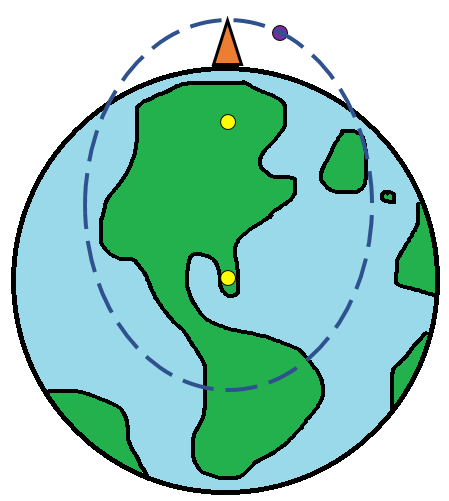
\includegraphics{Earth-Gravity.png}
\end{center}






We aren't drifting on this section.





















\begin{sectionOutcomes}
In this section, students will 

\begin{itemize}
\item analyze quadratic functions.
\item graph parabolas.
\item parameterize curves.
\end{itemize}
\end{sectionOutcomes}

\end{document}
